\documentclass{beamer}
\usetheme{Hannover}
\setbeamersize{sidebar width left=0pt}
\usepackage[T1, T2A]{fontenc}
\usepackage[utf8]{inputenc}
\usepackage[russian]{babel}
\usepackage{hyperref}
\usepackage{graphicx}
\graphicspath{ {../Images/} }

\author{Григорий Матюхин}
\date{\today}
\title{Лабораторная работа \textnumero5.}
\subtitle{Управление системными службами}

\begin{document}
\begin{frame}[plain]
	\titlepage
\end{frame}
\section{Цель работы}
\begin{frame}[plain]
	\frametitle{Цель работы}
	Получить навыки управления системными службами операционной системы посредством systemd.
\end{frame}

\section{Последовательность выполнения работы}
\subsection{Управление сервисами}
\begin{enumerate}
	\begin{frame}[plain]
		\frametitle{Управление сервисами}
		\item Проверьте статус службы Very Secure FTP:
		\item Установите службу Very Secure FTP: \\
		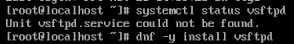
\includegraphics{1.png}
		\item Запустите службу Very Secure FTP:
		\item Проверьте статус службы Very Secure FTP: \\
		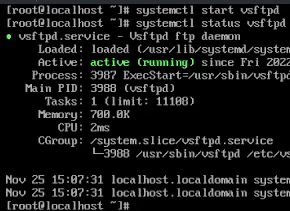
\includegraphics{2.png}
	\end{frame}
	\begin{frame}[plain]
		\item Добавьте службу Very Secure FTP в автозапуск при загрузке операционной системы, используя команду systemctl enable. Затем проверьте статус службы. \\
		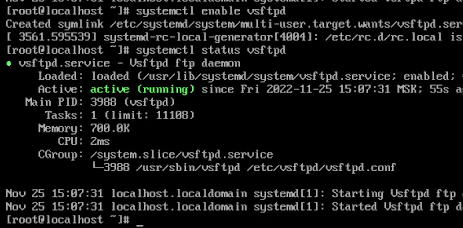
\includegraphics{3.png}
	\end{frame}
	\begin{frame}[plain]
		\item Удалите службу из автозапуска, используя команду systemctl disable, и снова проверьте её статус. \\
		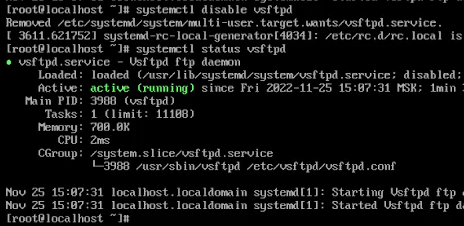
\includegraphics{4.png}
	\end{frame}
	\begin{frame}[plain]
		\item Выведите на экран символические ссылки, ответственные за запуск различных сервисов: \\
		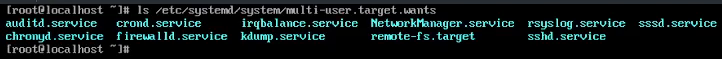
\includegraphics{5.png}
	\end{frame}
	\begin{frame}[plain]
		\item Снова добавьте службу Very Secure FTP в автозапуск и выведите на экран символические ссылки, ответственные за запуск различных сервисов. \\
		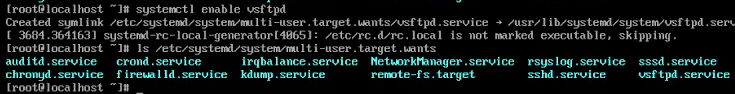
\includegraphics{6.png}
	\end{frame}
	\begin{frame}[plain]
		\item Снова проверьте статус службы Very Secure FTP:
		\item Выведите на экран список зависимостей юнита: \\
		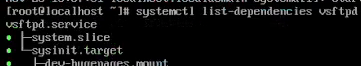
\includegraphics{7.png}
		\item Выведите на экран список юнитов, которые зависят от данного юнита: \\
		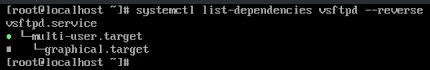
\includegraphics{8.png}
	\end{frame}
\end{enumerate}

\subsection{Конфликты юнитов}
\begin{enumerate}
	\begin{frame}[plain]
		\frametitle{Конфликты юнитов}
		\item Проверьте статус firewalld и iptables: \\
		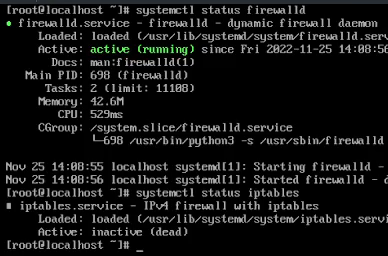
\includegraphics{9.png}
	\end{frame}
	\begin{frame}[plain]
		\item Попробуйте запустить firewalld и iptables: \\
		
\includegraphics{10.png}
	\end{frame}
	\begin{frame}[plain]
		\item Опишите настройки конфликтов для firewalld при наличии: \\
		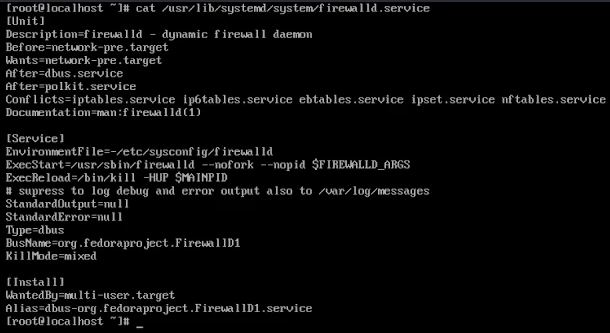
\includegraphics{11.png}
	\end{frame}
	\begin{frame}[plain]
		\item Опишите настройки конфликтов для iptables при наличии: \\
		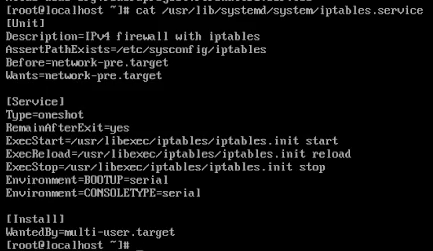
\includegraphics{12.png}
	\end{frame}
	\begin{frame}[plain]
		\item Выгрузите службу iptables и загрузите службу firewalld:
		\item Заблокируйте запуск iptables:
		\item Попробуйте запустить iptables:
		\item Попробуйте добавить iptables в автозапуск: \\
		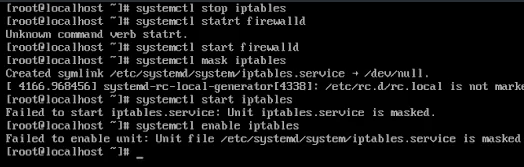
\includegraphics{13.png}
	\end{frame}
\end{enumerate}

\subsection{Изолируемые цели}
\begin{enumerate}
	\begin{frame}[plain]
		\frametitle{Изолируемые цели}
		\item Получите полномочия администратора. Перейдите в каталог systemd и найдите список всех целей, которые можно изолировать: \\
		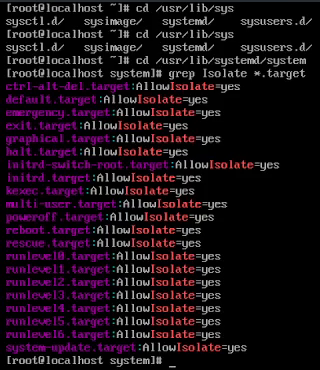
\includegraphics{14.png}
	\end{frame}
	\begin{frame}[plain]
		\item Переключите операционную систему в режим восстановления: \\
		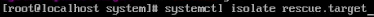
\includegraphics{15.png}
		\item Перезапустите операционную систему: \\
		
\includegraphics{16.png}
	\end{frame}
\end{enumerate}

\subsection{Цель по умолчанию}
\begin{enumerate}
	\begin{frame}[plain]
		\frametitle{Цель по умолчанию}
		\item Выведите на экран цель, установленную по умолчанию: \\
		\item Установаите другую цель как цель по умолчанию: \\
		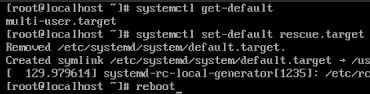
\includegraphics{17.png}
	\end{frame}
	\begin{frame}[plain]
		\item Перегрузите систему командой reboot. Убедитесь, что система загрузилась в установленном режиме:
		\item Верните предыдущую цель как цель по умолчанию: \\
		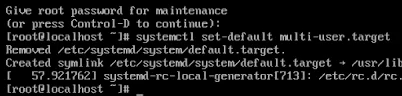
\includegraphics{18.png}
	\end{frame}
\end{enumerate}

\section{Вывод}
\begin{frame}[plain]
	\frametitle{Вывод}
	В ходе выполнения данной работы я получил навыки управления системными службами операционной системы посредством systemd.
\end{frame}

\end{document}
